\documentclass{beamer}
\usepackage[utf8]{inputenc}
\usepackage[T1]{fontenc}
\usepackage[english]{babel}
\usepackage{graphicx}
\usepackage{times}
\usepackage{algorithm}
\usepackage{algpseudocode}
\usepackage{amsmath}
\usepackage{amssymb}
\usepackage{tikz}
\usetikzlibrary{calc,through,backgrounds,positioning,fit}
\usetikzlibrary{shapes,arrows,shadows,calendar}
%\usetheme{Rochester}
%\usetheme{Berkeley}
%\usetheme{Copenhagen}
\usetheme{Warsaw}
\title{Beamer}
\author{A. Iksiński}
\institute{Wydział EAIiIB\\
	Katedra Informatyki Stosowanej}
\date{2015}
 \begin{document} 
 %-------------------------------------------------
\frame{\titlepage}
%-------------------------------------------------

\begin{frame}[fragile]    % fragile!!!, bo używamy verb
\frametitle{Algorytm} 
\begin{algorithmic}
\State $\triangleright$ \verb!ASSIGN! \pause
\State $\triangleright$ \verb!init(s) = s0;! \pause
\State $\triangleright$ \verb!next(s) := case! \pause
\ForAll {$si \in s$}\pause
\ForAll {$tk \in T$}\pause
\State $V_{ik} \gets \emptyset$\pause
\ForAll {$sj \in s$}\pause
\If {$(M_i,S_i)\xrightarrow{tk} (M_j,S_j) $}\pause
\State $V_{ik} \gets V_{ik} \cup \{sj\}$\pause
\EndIf\pause
\EndFor
\State $\triangleright$ \verb!s = si & action = tk:! \{$V_{ik}$ contents\};\pause
\EndFor
\EndFor
\State $\triangleright$ \verb!esac;!
\end{algorithmic}
 
\end{frame}
 
%--------------------------------------------------
 
\begin{frame}
\frametitle{Zadanie 5.1}
\tikzstyle{place}=[shape=circle, draw, minimum height=10mm]
\tikzstyle{trig}=[shape=circle, draw, dashed, minimum height=10mm]
\tikzstyle{trans}=[shape=rectangle, draw, minimum height=6mm, minimum width=12mm] 
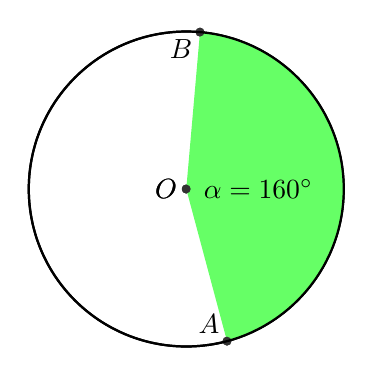
\begin{tikzpicture}[scale=1,inner sep=0.4mm]
\onslide<1->{
  \coordinate (O) at (0,0);
  \coordinate (A) at (-75:2cm);
  \coordinate (B) at (85:2cm);
  \node at (O) [circle,fill=black!80!white] {};
  \node at (O) [left=2pt] {$O$};
  \draw [thick] (O) circle (2cm);
}
\onslide<2->{
\node at (O) [circle,fill=black!80!white] {};
\node at (A) [circle,fill=black!80!white] {};
\node at (B) [circle,fill=black!80!white] {};
\node at (O) [left=2pt] {$O$};
\node at (A) [above left=2pt] {$A$};
\node at (B) [below left=2pt] {$B$};
}
\onslide<3->{
\fill[green!60!white] (O) -- (2,0) arc (0:85:2.0cm) -- cycle;
\fill[green!60!white] (O) -- (2,0) arc (0:-75:2.0cm) -- cycle;
\node at (O) [right=5pt] {$\alpha = 160^\circ$};	
\node at (O) [circle,fill=black!80!white] {};
\node at (A) [circle,fill=black!80!white] {};
\node at (B) [circle,fill=black!80!white] {};
\draw [thick] (O) circle (2cm);
}
\end{tikzpicture}
 
\end{frame}
 
%--------------------------------------------------
 
\begin{frame}
\frametitle{Kalendarz}
 
\begin{columns}
\column{0.45\textwidth}
\begin{block}{Styczeń 2015}
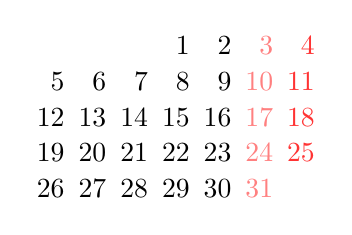
\begin{tikzpicture}[]
\calendar
[dates=2015-01-01 to 2015-01-31,week list]
if (Saturday) [red!50]
if (Sunday) [red!80];
\end{tikzpicture}
\end{block}
\column{0.5\textwidth}
\only<2>{
  \begin{block}{Luty 2015}
  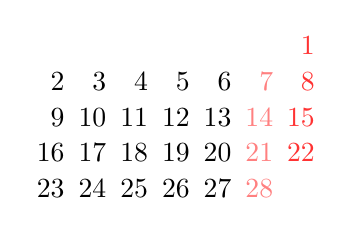
\begin{tikzpicture}[]
  \calendar
  [dates=2015-02-01 to 2015-02-28,week list]
  if (Saturday) [red!50]
  if (Sunday) [red!80];
  \end{tikzpicture}
  \end{block}
}
\only<3>{
	\begin{block}{Marzec 2015}
		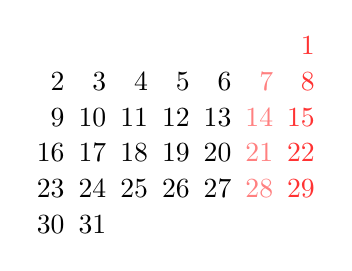
\begin{tikzpicture}[]
		\calendar
		[dates=2015-03-01 to 2015-03-31,week list]
		if (Saturday) [red!50]
		if (Sunday) [red!80];
		\end{tikzpicture}
	\end{block}
}
\only<4>{
	\begin{block}{Kwiecień 2015}
		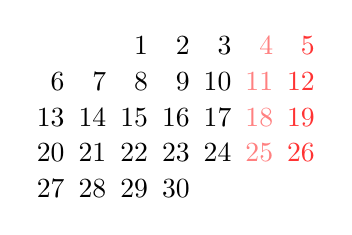
\begin{tikzpicture}[]
		\calendar
		[dates=2015-04-01 to 2015-04-30,week list]
		if (Saturday) [red!50]
		if (Sunday) [red!80];
		\end{tikzpicture}
	\end{block}
}
\end{columns}
\end{frame}
 
\end{document}